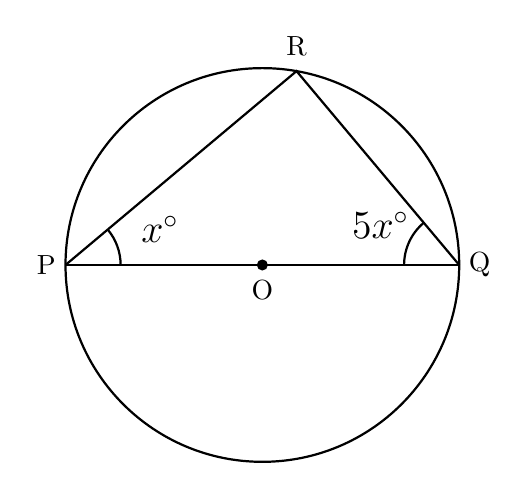
\begin{tikzpicture}[scale=1]

    % Define the radius of the circle
    \def\R{2.5}

    % Define the center of the circle
    \coordinate (O) at (0,0);

    % Define points P and Q on the circle such that PQ is a diameter
    \coordinate (P) at (-\R, 0);
    \coordinate (Q) at (\R, 0);

    % Define point R on the circle. 
    % Moved closer to the middle (top) to match the visual representation better.
    % We use 80 degrees so it's nearly central but retains a slight asymmetry.
    \coordinate (R) at (80:\R);

    % Draw the circle
    \draw[thick] (O) circle (\R);

    % Draw the diameter PQ
    \draw[thick] (P) -- (Q);

    % Draw the segments PR and QR to form the inscribed triangle
    \draw[thick] (P) -- (R) -- (Q);

    % Draw the center point O as a small filled circle
    \fill (O) circle (2pt);

    % Draw the angle arc at P
    \draw[thick] (P) ++(0:0.7) arc (0:40:0.7);

    % Draw the angle arc at Q
    \draw[thick] (Q) ++(180:0.7) arc (180:130:0.7);

    % Add the labels for the points exactly as shown in the image
    \node[left] at (P) {P};
    \node[right] at (Q) {Q};
    \node[above, yshift=2pt] at (R) {R};
    \node[below, yshift=-2pt] at (O) {O};

    % Add the angle measurements inside the triangle
    % Using \Large to make x and 5x bigger
    \node at (-1.3, 0.45) {\Large $x^\circ$};
    \node at (1.5, 0.5) {\Large $5x^\circ$};

\end{tikzpicture}